\documentclass[12pt,]{article}
\usepackage[utf8]{inputenc}
\usepackage[T1]{fontenc}
\usepackage{mathptmx}
\usepackage{geometry}
\usepackage{mathtools}
\usepackage[english]{babel}
\usepackage{graphicx}
\usepackage[os=win]{menukeys}
\usepackage[figurename=Gambar]{caption}
\usepackage{hyperref}
\usepackage{minted}
\usepackage{xcolor}
\usepackage{tikz}
\usepackage[yyyymmdd,hhmmss]{datetime}

\newcommand{\WindowsLogo}{\raisebox{-0.1em}{\includegraphics[height=0.8em]{winlogo/Windows_3_logo_simplified}}}
\newcommand{\PowerLogo}{\raisebox{-0.1em}{\includegraphics[height=0.8em]{winlogo/power}}}
\newcommand{\WinKey}{\keys{\WindowsLogo}}	
\newcommand{\PowerKey}{\keys{\PowerLogo}}

\newcommand{\ShowOsVersion}{
	\immediate\write18{\unexpanded{foo=`uname -sro` && echo "\\\verb${foo}" > tmp.tex}}
	\input{tmp}\immediate\write18{rm tmp.tex}
}

\newcommand{\ShowTexVersion}{
	\immediate\write18{\unexpanded{foo=`pdflatex -version | head -n1` && echo "\\\verb${foo}" > tmp.tex}}
	\input{tmp}\immediate\write18{rm tmp.tex}
}	

\addto\captionsenglish{\renewcommand{\contentsname}{Daftar Isi}}

\hypersetup{
	colorlinks=true, %set true if you want colored links
	linktoc=all,     %set to all if you want both sections and subsections linked
	linkcolor=blue,  %choose some color if you want links to stand out
}

\geometry{
	a4paper,
	left=15mm,
	right=10mm,
	top=10mm,
	bottom=10mm,
}

\title{\Large \bf
	Tutorial Penggunaan HTS (Grapheme)
}

\author{Achmadi ST MT}

\date{}

\definecolor{LightGray}{gray}{0.9}

\usetikzlibrary{trees}

\tikzstyle{every node}=[draw=black,thick,anchor=west]
\tikzstyle{selected}=[draw=red,fill=red!30]
\tikzstyle{optional}=[dashed,fill=gray!50]

\begin{document}
	
	\maketitle
	\thispagestyle{empty}
	\pagestyle{empty}
	
	\begin{figure}[!ht]
		\centering
		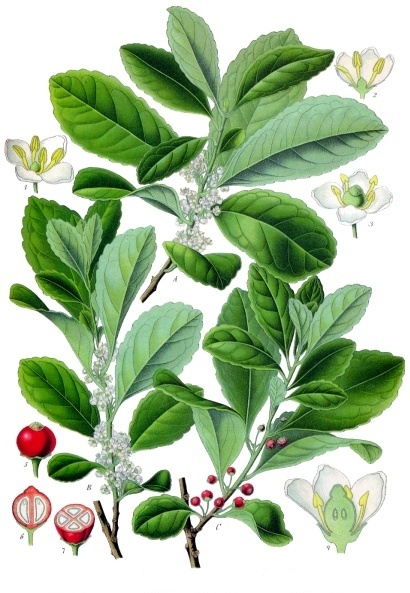
\includegraphics[width=250pt]{yerba.png}
	\end{figure}
	
	\vspace*{175px}
	\noindent This book written using: \\
	OS : \ShowOsVersion \\
	TeX : \ShowTexVersion \\
	Update: {\today} at \currenttime \\
	
	\noindent Document Tex Source:\\
	\url{https://github.com/mekatronik-achmadi/hts_grapheme/blob/master/panduan/panduan.tex}
	
	\newpage
	\mbox{}
	
	\newpage
	(catatan: Daftar Isi dan Index bisa diklik)
	\tableofcontents
	
	\newpage
	\mbox{}
	
	\newpage
	\section{Requirement}
	
	Untuk menjalankan isi panduan ini diperlukan antara lain:
	
	\subsection{Sistem Komputer}
	Di sisi sistem komputer, membutuhkan minimal:
	
	\begin{itemize}
		\item Komputer PC atau Laptop dengan pendingin bagus.
		\item Multi-Core Processor dengan clock minimal 2.5GHz
		\item RAM PC3 dengan kapasitas minimal 8GB
		\item Sistem Operasi berbasis Linux atau Unix-\textit{like}.\\
		Direkomendasikan Arch-Linux atau Ubuntu-MATE.
		Tidak direkomendasikan MacOS atau BSD-\textit{family} lainnya.
		\item Koneksi internet minimal stabil 1MBps (untuk download sources).
	\end{itemize}
	
	\subsection{Pengguna}
	Sedangkan untuk pengguna sendiri, membutuhkan minimal:
	
	\begin{itemize}
		\item Memahami akses shell atau terminal ke suatu alamat directory/folder.
		\item Memahami struktur directory/folder dan paham pindah alamatnya.
		\item Cukup familiar dengan bahasa Unix shell (Bash).
		\item Cukup familiar dengan instalasi paket di distro yang digunakan.
		\item Cukup kenal dengan bahasa bantu Perl dan Python.
		\item Tidak alergi pemrograman.
		\item Paham menggunakan Google dalam English.
		\item Tidak malas untuk troubleshot sendiri.
	\end{itemize}

	Jika semua kebutuhan ini terpenuhi, maka kemungkinan besar anda mampu menggunakan panduan ini.
	Jika tidak, jangan menyerah, semua kesulitan akan berakhir, baik dengan memang selesai dan sukses, atau tinggalkan saja jika sudah menyerah.
	
	\newpage
	\section{Instalasi Tools}.
	
	Berikut adalah instalasi semua tools yang dibutuhkan secara runtut.
	
	\subsection{Download Sources}
	
	Berikut download URL (update Juni 2019) untuk semua sources yang dibutuhkan.
	Semua teks link dibawah ini dapat diklik dan otomatis membuka webrowser menuju URL yang diklik.
	
	
	\subsubsection{Free Open-Source}
	
	Semua paket open-sources berikut dapat didownload dengan bebas.
	
	\begin{itemize}
		\item festival-2.5.0-release.tar.gz.\\
		\url{http://www.festvox.org/packed/festival/2.5/festival-2.5.0-release.tar.gz}
		
		\item speech\_tools-2.5.0-release.tar.gz \\
		\url{http://www.festvox.org/packed/festival/2.5/speech_tools-2.5.0-release.tar.gz}
		
		\item festvox-2.8.0-release.tar.gz.\\
		\url{http://www.festvox.org/packed/festvox/2.8/festvox-2.8.0-release.tar.gz}
		
		\item festlex\_CMU.tar.gz, festlex\_OALD.tar.gz, dan festlex\_POSLEX.tar.gz. \\
		\url{http://www.festvox.org/packed/festival/2.5/festlex_CMU.tar.gz}\\
		\url{http://www.festvox.org/packed/festival/2.5/festlex_OALD.tar.gz}\\
		\url{http://www.festvox.org/packed/festival/2.5/festlex_POSLEX.tar.gz}
		
		\item festvox\_kallpc16k.tar.gz dan festvox\_rablpc16k.tar.gz \\
		\url{http://www.festvox.org/packed/festival/2.5/voices/festvox_kallpc16k.tar.gz}\\
		\url{http://www.festvox.org/packed/festival/2.5/voices/festvox_rablpc16k.tar.gz}
		
		\item festvox\_don.tar.gz dan  festvox\_kedlpc16k.tar.gz\\
		\url{http://www.cstr.ed.ac.uk/downloads/festival/1.95/festvox_don.tar.gz} \\
		\url{http://www.cstr.ed.ac.uk/downloads/festival/1.95/festvox_kedlpc16k.tar.gz}
		
		\item festvox\_cmu\_us\_*\_cg.tar.gz. \\
		\url{http://www.festvox.org/packed/festival/2.5/voices/festvox_cmu_us_aew_cg.tar.gz}\\
		\url{http://www.festvox.org/packed/festival/2.5/voices/festvox_cmu_us_ahw_cg.tar.gz}\\
		\url{http://www.festvox.org/packed/festival/2.5/voices/festvox_cmu_us_aup_cg.tar.gz}\\
		\url{http://www.festvox.org/packed/festival/2.5/voices/festvox_cmu_us_awb_cg.tar.gz}\\
		\url{http://www.festvox.org/packed/festival/2.5/voices/festvox_cmu_us_axb_cg.tar.gz}\\
		\url{http://www.festvox.org/packed/festival/2.5/voices/festvox_cmu_us_bdl_cg.tar.gz}\\
		\url{http://www.festvox.org/packed/festival/2.5/voices/festvox_cmu_us_clb_cg.tar.gz}\\
		\url{http://www.festvox.org/packed/festival/2.5/voices/festvox_cmu_us_eey_cg.tar.gz}\\
		\url{http://www.festvox.org/packed/festival/2.5/voices/festvox_cmu_us_fem_cg.tar.gz}\\
		\url{http://www.festvox.org/packed/festival/2.5/voices/festvox_cmu_us_gka_cg.tar.gz}\\
		\url{http://www.festvox.org/packed/festival/2.5/voices/festvox_cmu_us_jmk_cg.tar.gz}\\
		\url{http://www.festvox.org/packed/festival/2.5/voices/festvox_cmu_us_ksp_cg.tar.gz}\\
		\url{http://www.festvox.org/packed/festival/2.5/voices/festvox_cmu_us_ljm_cg.tar.gz}\\
		\url{http://www.festvox.org/packed/festival/2.5/voices/festvox_cmu_us_lnh_cg.tar.gz}\\
		\url{http://www.festvox.org/packed/festival/2.5/voices/festvox_cmu_us_rms_cg.tar.gz}\\
		\url{http://www.festvox.org/packed/festival/2.5/voices/festvox_cmu_us_rxr_cg.tar.gz}\\
		\url{http://www.festvox.org/packed/festival/2.5/voices/festvox_cmu_us_slp_cg.tar.gz}\\
		\url{http://www.festvox.org/packed/festival/2.5/voices/festvox_cmu_us_slt_cg.tar.gz}
		
		\item HTS-2.3\_for\_HTK-3.4.1.tar.bz2 \\
		\url{http://hts.sp.nitech.ac.jp/archives/2.3/HTS-2.3_for_HTK-3.4.1.tar.bz2}
		
		\item hts\_engine\_API-1.10.tar.gz \\
		\url{http://downloads.sourceforge.net/hts-engine/hts_engine_API-1.10.tar.gz}
		
		\item SPTK-3.10.tar.gz \\
		\url{http://downloads.sourceforge.net/sp-tk/SPTK-3.10.tar.gz}

		\item flite-2.0.0-release.tar.bz2 \\
		\url{http://festvox.org/flite/packed/flite-2.0/flite-2.0.0-release.tar.bz2}
	\end{itemize}
	
	\subsubsection{Limited Open-Sources}
	
	Semua paket open-sources berikut dapat didownload hanya dengan hak akses khusus.
	
	\begin{itemize}
		\item HTK-3.4.1.tar.gz \\
		\url{http://htk.eng.cam.ac.uk/ftp/software/HTK-3.4.1.tar.gz}
		
		\item HTK-samples-3.4.1.tar.gz \\
		\url{http://htk.eng.cam.ac.uk/ftp/software/HTK-samples-3.4.1.tar.gz}
		
		\item HDecode-3.4.1.tar.gz \\
		\url{http://htk.eng.cam.ac.uk/prot-docs/hdecode.shtml}
		
		
	\end{itemize}

	\subsection{Instalasi Paket Dasar}
	
	Selanjutnya adalah instalasi kebutuhan dasar yang telah tersedia di repository distro yang anda pakai.
	Paket yang dibutuhkan adalah:
	
	\begin{itemize}
		\item compiler-toolchain atau build-system.
		\item editor cli gawk.
		\item alternatif shell csh.
		\item pustaka pemrograman libx11.
		\item pustaka pemrograman ncurses5.
		\item sound processor sox.
	\end{itemize}

	Untuk instalasi ini, anda mungkin akan butuh koneksi internet dan hak akses root/sudo. \\
	
	Berikut perintah untuk instalasi di distro Ubuntu:
	\begin{minted}[frame=lines,framesep=2mm,fontsize=\footnotesize,bgcolor=LightGray]{bash}
sudo apt-get install csh gawk sox libx11-dev gcc-multilib libncurses5-dev
	\end{minted}
	
	Untuk distro Arch-Linux:
	\begin{minted}[frame=lines,framesep=2mm,fontsize=\footnotesize,bgcolor=LightGray]{bash}
sudo pacman -S tcsh gawk sox libx11 gcc-multilib 
	\end{minted}
	
	ditambah paket ncurses5-compat-libs dari AUR:\\
	\url{https://aur.archlinux.org/packages/ncurses5-compat-libs/}
	
	\begin{minted}[frame=lines,framesep=2mm,fontsize=\footnotesize,bgcolor=LightGray]{bash}
sudo pacman -U ncurses5-compat-libs*
	\end{minted}
	
	\newpage
	\subsection{Persiapan}
	
	Berikut langkah persiapan instalasi.
	
	\begin{enumerate}
		\item buat folder yang berisi semua paket source yang telah dikumpulkan.
		Contoh disini adalah di alamat \textbf{\textasciitilde/HTS/install}.
		
		\item Salin semua paket source ke dalam folder tersebut.
		
		\item Tentukan alamat folder tujuan instalasi.
		Contoh disini adalah di alamat \textbf{\textasciitilde/.hts\_sptk}
		
		\item Buka jendela terminal baru.
		
		\item Masukkan variabel lingkungan untuk alamat paket sources dan alamat tujuan instalasi.
		\begin{minted}[frame=lines,framesep=2mm,fontsize=\footnotesize,bgcolor=LightGray]{bash}
export SOURCE_DIR=~/HTS/install
export TARGET_DIR=~/.hts_sptk
		\end{minted}
		
		\item Check file di folder paket sumber.
		\begin{minted}[frame=lines,framesep=2mm,fontsize=\footnotesize,bgcolor=LightGray]{bash}
ls -1 $SOURCE_DIR
		\end{minted}
		
		dimana hasil yang diharapkan.
	\begin{minted}[frame=lines,framesep=2mm,fontsize=\footnotesize,bgcolor=LightGray]{bash}
festival-2.5.0-release.tar.gz
festlex_CMU.tar.gz
festlex_OALD.tar.gz
festlex_POSLEX.tar.gz
festvox-2.8.0-release.tar.gz
festvox_cmu_us_ahw_cg.tar.gz
festvox_cmu_us_aup_cg.tar.gz
festvox_cmu_us_awb_arctic_hts.tar.gz
festvox_cmu_us_awb_cg.tar.gz
festvox_cmu_us_axb_cg.tar.gz
festvox_cmu_us_bdl_cg.tar.gz
festvox_cmu_us_clb_cg.tar.gz
festvox_cmu_us_fem_cg.tar.gz
festvox_cmu_us_gka_cg.tar.gz
festvox_cmu_us_jmk_cg.tar.gz
festvox_cmu_us_ksp_cg.tar.gz
festvox_cmu_us_rms_cg.tar.gz
festvox_cmu_us_rxr_cg.tar.gz
festvox_cmu_us_slt_cg.tar.gz
festvox_don.tar.gz
festvox_kallpc16k.tar.gz
festvox_kedlpc16k.tar.gz
festvox_rablpc16k.tar.gz
flite-2.0.0-release.tar.bz2
HDecode-3.4.1.tar.gz
HTK-3.4.1.tar.gz
HTK-samples-3.4.1.tar.gz
HTS-2.3_for_HTK-3.4.1.tar.bz2
hts_engine_API-1.10.tar.gz
speech_tools-2.5.0-release.tar.gz
SPTK-3.10.tar.gz
	\end{minted}
	
	\newpage
	\item buat folder tujuan.
	\begin{minted}[frame=lines,framesep=2mm,fontsize=\footnotesize,bgcolor=LightGray]{bash}
mkdir -p $TARGET_DIR
	\end{minted}
	
	\item Anda dapat menutup jendela terminal/shell.
		
	\end{enumerate}

	\subsection{Extraksi}
	
	Selanjutnya adalah ekstraksi semua paket sources.
	Berikut langkahnya:
	
	\begin{enumerate}
		\item Buka jendela terminal baru.
		
		\item Masukkan variabel lingkungan untuk alamat paket sources dan alamat tujuan instalasi.
		\begin{minted}[frame=lines,framesep=2mm,fontsize=\footnotesize,bgcolor=LightGray]{bash}
export SOURCE_DIR=~/HTS/install
export TARGET_DIR=~/.hts_sptk
		\end{minted}
		
		\item Masukkan perintah ekstraksi untuk semua paket:
		\begin{minted}[frame=lines,framesep=2mm,fontsize=\footnotesize,bgcolor=LightGray]{bash}
tar zxvf $SOURCE_DIR/SPTK-3.10.tar.gz -C $TARGET_DIR
tar zxvf $SOURCE_DIR/HTK-3.4.1.tar.gz -C $TARGET_DIR
tar zxvf $SOURCE_DIR/HDecode-3.4.1.tar.gz -C $TARGET_DIR
tar zxvf $SOURCE_DIR/HTK-samples-3.4.1.tar.gz -C $TARGET_DIR
tar jxvf $SOURCE_DIR/HTS-2.3_for_HTK-3.4.1.tar.bz2 -C $TARGET_DIR
tar zxvf $SOURCE_DIR/hts_engine_API-1.10.tar.gz -C $TARGET_DIR
tar zxvf $SOURCE_DIR/speech_tools-2.5.0-release.tar.gz -C $TARGET_DIR
tar zxvf $SOURCE_DIR/festival-2.5.0-release.tar.gz -C $TARGET_DIR
tar zxvf $SOURCE_DIR/festlex_CMU.tar.gz -C $TARGET_DIR
tar zxvf $SOURCE_DIR/festlex_POSLEX.tar.gz -C $TARGET_DIR
tar zxvf $SOURCE_DIR/festlex_OALD.tar.gz -C $TARGET_DIR
tar zxvf $SOURCE_DIR/festvox_kallpc16k.tar.gz -C $TARGET_DIR
tar zxvf $SOURCE_DIR/festvox_rablpc16k.tar.gz -C $TARGET_DIR
tar zxvf $SOURCE_DIR/festvox_kedlpc16k.tar.gz -C $TARGET_DIR
tar zxvf $SOURCE_DIR/festvox_cmu_us_ahw_cg.tar.gz -C $TARGET_DIR
tar zxvf $SOURCE_DIR/festvox_cmu_us_aup_cg.tar.gz -C $TARGET_DIR
tar zxvf $SOURCE_DIR/festvox_cmu_us_awb_arctic_hts.tar.gz -C $TARGET_DIR
tar zxvf $SOURCE_DIR/festvox_cmu_us_awb_cg.tar.gz -C $TARGET_DIR
tar zxvf $SOURCE_DIR/festvox_cmu_us_axb_cg.tar.gz -C $TARGET_DIR
tar zxvf $SOURCE_DIR/festvox_cmu_us_bdl_cg.tar.gz -C $TARGET_DIR
tar zxvf $SOURCE_DIR/festvox_cmu_us_clb_cg.tar.gz -C $TARGET_DIR
tar zxvf $SOURCE_DIR/festvox_cmu_us_fem_cg.tar.gz -C $TARGET_DIR
tar zxvf $SOURCE_DIR/festvox_cmu_us_gka_cg.tar.gz -C $TARGET_DIR
tar zxvf $SOURCE_DIR/festvox_cmu_us_jmk_cg.tar.gz -C $TARGET_DIR
tar zxvf $SOURCE_DIR/festvox_cmu_us_ksp_cg.tar.gz -C $TARGET_DIR
tar zxvf $SOURCE_DIR/festvox_cmu_us_rms_cg.tar.gz -C $TARGET_DIR
tar zxvf $SOURCE_DIR/festvox_cmu_us_rxr_cg.tar.gz -C $TARGET_DIR
tar zxvf $SOURCE_DIR/festvox_cmu_us_slt_cg.tar.gz -C $TARGET_DIR
tar zxvf $SOURCE_DIR/festvox-2.8.0-release.tar.gz -C $TARGET_DIR
tar jxvf $SOURCE_DIR/flite-2.0.0-release.tar.bz2 -C $TARGET_DIR
ls -1 $TARGET_DIR
		\end{minted}
		
		\newpage
		\item setelah baris perintah terakhir dieksekusi, maka hasil yang diharapkan:
		\begin{minted}[frame=lines,framesep=2mm,fontsize=\footnotesize,bgcolor=LightGray]{bash}
ChangeLog
COPYING
festival
festvox
flite-2.0.0-release
htk
HTS-2.3_for_HTK-3.4.1.patch
HTS_Document.pdf
hts_engine_API-1.10
INSTALL
README
samples
speech_tools
SPTK-3.10
		\end{minted}
		
		\item Anda dapat menutup jendela terminal/shell.
		
	\end{enumerate}

	\subsection{Build dan Install}
	
	Selanjutnya adalah langkah instalasi setiap komponen.
	
	\begin{enumerate}
		\item Buka jendela terminal baru.
		
		\item Masukkan variabel lingkungan untuk alamat paket sources dan alamat tujuan instalasi.
		\begin{minted}[frame=lines,framesep=2mm,fontsize=\footnotesize,bgcolor=LightGray]{bash}
export SOURCE_DIR=~/HTS/install
export TARGET_DIR=~/.hts_sptk
		\end{minted}
		
		\item Jendela teminal/shell ini yang akan digunakan untuk instalasi semua komponen.
		Jangan menutup atau membuka jendela baru.
		
		\item Berikutnya perintah instalasi tiap komponen.
	\end{enumerate}

	\subsubsection{SPTK}
	\begin{minted}[frame=lines,framesep=2mm,fontsize=\footnotesize,bgcolor=LightGray]{bash}
cd $TARGET_DIR/SPTK-3.10
./configure --prefix=$TARGET_DIR
make all
make install
	\end{minted}
	
	\subsubsection{HTK}
	
	Untuk Ubuntu:
	\begin{minted}[frame=lines,framesep=2mm,fontsize=\footnotesize,bgcolor=LightGray]{bash}
cd $TARGET_DIR/htk
patch -p1 < ../HTS-2.3_for_HTK-3.4.1.patch
./configure CFLAGS=-DARCH=linux --prefix=$TARGET_DIR
make all
make install
make hdecode
make install-hdecode
	\end{minted}
	
	\newpage
	Untuk Arch-Linux:
	\begin{minted}[frame=lines,framesep=2mm,fontsize=\footnotesize,bgcolor=LightGray]{bash}
cd $TARGET_DIR/htk
patch -p1 < ../HTS-2.3_for_HTK-3.4.1.patch
./configure --prefix=$TARGET_DIR
make all
make install
make hdecode
make install-hdecode
	\end{minted}
	
	\subsubsection{HTS}
	\begin{minted}[frame=lines,framesep=2mm,fontsize=\footnotesize,bgcolor=LightGray]{bash}
cd $TARGET_DIR/hts_engine_API-1.10
./configure --prefix=$TARGET_DIR
make all
make install
	\end{minted}
	
	\subsubsection{Flite}
	\begin{minted}[frame=lines,framesep=2mm,fontsize=\footnotesize,bgcolor=LightGray]{bash}
cd $TARGET_DIR/flite-2.0.0-release
./configure --prefix=$TARGET_DIR
make all
make install
	\end{minted}

	\subsubsection{Speech-Tools}
	\begin{minted}[frame=lines,framesep=2mm,fontsize=\footnotesize,bgcolor=LightGray]{bash}
cd $TARGET_DIR/speech_tools
./configure --prefix=$TARGET_DIR
make all
make install
	\end{minted}
	
	\subsubsection{Festival}
	\begin{minted}[frame=lines,framesep=2mm,fontsize=\footnotesize,bgcolor=LightGray]{bash}
cd $TARGET_DIR/festival
./configure --prefix=$TARGET_DIR
make all
make install
	\end{minted}
	
	\subsubsection{FestVox}
	\begin{minted}[frame=lines,framesep=2mm,fontsize=\footnotesize,bgcolor=LightGray]{bash}
cd $TARGET_DIR/festvox
./configure --prefix=$TARGET_DIR
sed -i "s#NUL)#NULL)#g" src/vc/src/sub/gmm_sub.cc
make all
	\end{minted}
	
	Instalasi seluruh komponen telah selesai, maka anda menutup jendela terminal/shell.
	
	\newpage
	\subsection{Tools EnVars}
	
	Selanjutnya untuk dapat menggunakan tools yang telah diinstal,
	anda perlu men-set variable lingkungan (Environment Variables atau EnVars),
	sehingga shell/terminal dapat mengakses tools tersebut.
	
	Jika contoh dalam panduan ini menggunakan alamat instalasi \textbf{\textasciitilde/.hts\_sptk},
	maka perintah set envars:
	
	\begin{minted}[frame=lines,framesep=2mm,fontsize=\footnotesize,bgcolor=LightGray]{bash}
export TOOLS_DIR=~/.hts_sptk

export PATH=$TOOLS_DIR/bin:$PATH
export PATH=$TOOLS_DIR/festival/bin:$PATH
export PATH=$TOOLS_DIR/speech_tools/bin:$PATH

export FESTVOXDIR=$TOOLS_DIR/festvox
export FESTDIR=$TOOLS_DIR/festival
export ESTDIR=$TOOLS_DIR/speech_tools

export PATH=$FESTDIR/examples:$PATH
	\end{minted}
	
	Perintah ini wajib dijalankan setiap kali anda menggunakan terminal/shell yang baru untuk menjalankan tools yang telah diinstal.

	\subsection{Uji Demo}
	
	Setelah proses instalasi selesai, maka dapat dilakukan pengujian paket Demo untuk memastikan instalasi telah sukses.
	
	Sebelum menguji, download terlebih dahulu paket Demo untuk HTS 2.3 Speaker dependent:\\
	\url{http://hts.sp.nitech.ac.jp/archives/2.3/HTS-demo_CMU-ARCTIC-SLT.tar.bz2}
	
	\subsubsection{Run Demo}
	Berikut langkah menjalankan demo:
	
	\begin{enumerate}
		\item Buka jendela terminal dimana file \textbf{HTS-demo\_CMU-ARCTIC-SLT.tar.bz2} berada.
		
		\item Extract paket demo ke suatu folder (sebagai contoh \textbf{demo\_hts}), kemudian pindah ke alamat tersebut.
		\begin{minted}[frame=lines,framesep=2mm,fontsize=\footnotesize,bgcolor=LightGray]{bash}
mkdir -p demo_hts/
tar jxvf HTS-demo_CMU-ARCTIC-SLT.tar.bz2 -C demo_hts/
cd demo_hts/HTS-demo_CMU-ARCTIC-SLT/
		\end{minted}
		
		\item Panggil Envars tools:
		\begin{minted}[frame=lines,framesep=2mm,fontsize=\footnotesize,bgcolor=LightGray]{bash}
export TOOLS_DIR=~/.hts_sptk

export PATH=$TOOLS_DIR/bin:$PATH
export PATH=$TOOLS_DIR/festival/bin:$PATH
export PATH=$TOOLS_DIR/speech_tools/bin:$PATH

export FESTVOXDIR=$TOOLS_DIR/festvox
export FESTDIR=$TOOLS_DIR/festival
export ESTDIR=$TOOLS_DIR/speech_tools

export PATH=$FESTDIR/examples:$PATH
		\end{minted}
		
		\newpage
		\item Set nama file log dengan jam dan tanggal.
		\begin{minted}[frame=lines,framesep=2mm,fontsize=\footnotesize,bgcolor=LightGray]{bash}
export NMFILE="$(date +'%d%m%Y_%H%M')"
		\end{minted}
		
		\item Konfigurasi alamat tools untuk skrip demo:
		\begin{minted}[frame=lines,framesep=2mm,fontsize=\footnotesize,bgcolor=LightGray]{bash}
chmod a+x configure
./configure \
--with-fest-search-path=$TOOLS_DIR/festival/examples \
--with-sptk-search-path=$TOOLS_DIR/bin \
--with-hts-search-path=$TOOLS_DIR/bin \
--with-hts-engine-search-path=$TOOLS_DIR/bin \
DATASET=cmu_us_arctic SPEAKER=slt
		\end{minted}

		\item Persiapan data dan skrip.
		Alamat dataset ada di \textbf{data/\{raw,txt,utts\}}.
		\begin{minted}[frame=lines,framesep=2mm,fontsize=\footnotesize,bgcolor=LightGray]{bash}
make all 2>&1 | tee log_prepare_$NMFILE.txt
		\end{minted}
		
		Tunggu proses selesai dan muncul bash-prompt.
		Selain tampil di terminal, proses akan tercatat di file log\_prepare\_jamtanggal.txt

		\item Synthesis kalimat yang ada di \textbf{data/labels/gen/}.
		\begin{minted}[frame=lines,framesep=2mm,fontsize=\footnotesize,bgcolor=LightGray]{bash}
scriptpath=$(pwd)
perl scripts/Training.pl $scriptpath/scripts/Config.pm 2>&1 | tee log_synthesis_$NMFILE.txt
		\end{minted}
		
		Tunggu proses selesai dan muncul bash-prompt.
		Selain tampil di terminal, proses akan tercatat di file log\_synthesis\_jamtanggal.txt
		
		\item Hasil synthesis dapat di cek di folder \textbf{gen/qst001/ver1/\{1mix,2mix,hts\_engine,stc\}}
		
	\end{enumerate}
	
	\newpage
	\subsubsection{Tracking Proses Synthesis}.
	
	Selama proses synthesis berjalan, anda dapat menjejak (\textit{tracking}) sudah sampai tahap mana proses berlangsung.
	Tracking dilakukan dengan menilik tahapan "Start" yang tercatat di file log\_synthesis\_jamtanggal.txt.
	
	Sebagai contoh file log terakhir atau sedang berlangsung memiliki nama \textbf{log\_synthesis\_10062019\_1444.txt}.
	Berikut langkah tracking:
	
	\begin{enumerate}
		\item Buka jendela terminal/shell di alamat file \textbf{log\_synthesis\_10062019\_1444.txt} berada.
		
		\item Perintah untuk print menampilkan tahapan synthesis yang sudah selesai dan yang terakhir sedang berjalan:
		\begin{minted}[frame=lines,framesep=2mm,fontsize=\footnotesize,bgcolor=LightGray]{bash}
cat log_synthesis_10062019_1444.txt | grep "Start"
		\end{minted}

		\item Sebagai pembanding, dapat dibandingkan dengan konten konfigurasi di file \textbf{scripts/Config.pm}.
		\begin{minted}[frame=lines,framesep=2mm,fontsize=\footnotesize,bgcolor=LightGray]{bash}
tail -n35 scripts/Config.pm
		\end{minted}
		
	\end{enumerate}

	Jika proses synthesis berhenti di tengah jalan, proses dapat di ulang tanpa harus dari awal,
	dengan cara memanipulasi nilai 0 atau 1 pada segmen \textbf{SWITCH} pada file \textbf{scripts/Config.pm}.
	
	\begin{minted}[frame=lines,framesep=2mm,fontsize=\footnotesize,bgcolor=LightGray]{bash}
# Switch ================================
$MKEMV = 1; # preparing environments
$HCMPV = 1; # computing a global variance
$IN_RE = 1; # initialization & reestimation
$MMMMF = 1; # making a monophone mmf
$ERST0 = 1; # embedded reestimation (monophone)
$MN2FL = 1; # copying monophone mmf to fullcontext one
$ERST1 = 1; # embedded reestimation (fullcontext)
$CXCL1 = 1; # tree-based context clustering
$ERST2 = 1; # embedded reestimation (clustered)
$UNTIE = 1; # untying the parameter sharing structure
$ERST3 = 1; # embedded reestimation (untied)
$CXCL2 = 1; # tree-based context clustering
$ERST4 = 1; # embedded reestimation (re-clustered)
$FALGN = 1; # forced alignment for no-silent GV
$MCDGV = 1; # making global variance
$MKUNG = 1; # making unseen models (GV)
$TMSPF = 1; # training modulation spectrum-based postfilter
$MKUN1 = 1; # making unseen models (1mix)
$PGEN1 = 1; # generating speech parameter sequences (1mix)
$WGEN1 = 1; # synthesizing waveforms (1mix)
$CONVM = 1; # converting mmfs to the hts_engine file format
$ENGIN = 1; # synthesizing waveforms using hts_engine
$SEMIT = 1; # semi-tied covariance matrices
$MKUNS = 1; # making unseen models (stc)
$PGENS = 1; # generating speech parameter sequences (stc)
$WGENS = 1; # synthesizing waveforms (stc)
$UPMIX = 1; # increasing the number of mixture components (1mix -> 2mix)
$ERST5 = 1; # embedded reestimation (2mix)
$MKUN2 = 1; # making unseen models (2mix)
$PGEN2 = 1; # generating speech parameter sequences (2mix)
$WGEN2 = 1; # synthesizing waveforms (2mix)
	\end{minted}

	\newpage
	\subsection{Modifikasi Grapheme}
	
	Panduan ini akan membahas modifikasi Grapheme untuk menyesuaikan dengan bahasa Indonesia.
	
	\begin{enumerate}
		\item Buka jendela terminal/shell baru.
		
		\item Panggil Envars tools:
		\begin{minted}[frame=lines,framesep=2mm,fontsize=\footnotesize,bgcolor=LightGray]{bash}
export TOOLS_DIR=~/.hts_sptk

export PATH=$TOOLS_DIR/bin:$PATH
export PATH=$TOOLS_DIR/festival/bin:$PATH
export PATH=$TOOLS_DIR/speech_tools/bin:$PATH

export FESTVOXDIR=$TOOLS_DIR/festvox
export FESTDIR=$TOOLS_DIR/festival
export ESTDIR=$TOOLS_DIR/speech_tools

export PATH=$FESTDIR/examples:$PATH
		\end{minted}
		
		\item ganti deskripsi karakter di \textbf{\$FESTVOXDIR/src/grapheme/sampa.table}
		\begin{itemize}		
			\item "J" ke "j" pada baris 55.
			\item "j" ke "y" pada baris 82.
		\end{itemize}
	
		Perintahnya:
		\begin{minted}[frame=lines,framesep=2mm,fontsize=\footnotesize,bgcolor=LightGray]{bash}
sed -i "55s#( J#( j#" $FESTVOXDIR/src/grapheme/sampa.table
sed -i "82s#( j#( y#" $FESTVOXDIR/src/grapheme/sampa.table
		\end{minted}
		
		\item ganti asosiasi karakter di \textbf{\$FESTVOXDIR/src/grapheme/unicode\_sampa\_mapping.scm}
		\begin{itemize}
			\item A ke a di baris 26
			\item ch ke c di baris 28
			\item dZ ke j di baris 35
			\item j ke y di baris 50
		\end{itemize}
		
		Perintahnya:
		\begin{minted}[frame=lines,framesep=2mm,fontsize=\footnotesize,bgcolor=LightGray]{bash}
sed -i "26s#(( A )))#(( a )))#" $FESTVOXDIR/src/grapheme/unicode_sampa_mapping.scm
sed -i "28s#(( ch )))#(( c )))#" $FESTVOXDIR/src/grapheme/unicode_sampa_mapping.scm

sed -i "35s#(( dZ )))#(( j )))#" $FESTVOXDIR/src/grapheme/unicode_sampa_mapping.scm
sed -i "50s#(( j )))#(( y )))#" $FESTVOXDIR/src/grapheme/unicode_sampa_mapping.scm
		\end{minted}
		
	\end{enumerate}

	\newpage
	\mbox{}
	
	\newpage
	\section{Data Preparation}
	
	Panduan berikut untuk menyiapkan data rekaman untuk proses synthesis.
	
	\subsection{Minimum Data}
	
	Minimum data yang dibutuhkan secara standar adalah:
	\begin{itemize}
		\item semua file rekaman wav untuk synthesis. 
		Contoh disini memiliki nama vibid\_fena\_xxxx.wav
		
		\item satu file text berisi transkripsi rekaman wav sebelumnya.
		Contoh disini memiliki nama vibid\_fena.txt
	\end{itemize}

	\textbf{Perhatikan}:
	\begin{itemize}
		\item Pastikan urutan text sesuai urutan angka file wav dan sesuai.
		\item Pastikan tidak ada wav tanpa text bersesuaian atau sebaliknya.
	\end{itemize}

	\subsection{Build Text}
	
	Berikut langkah untuk membuat teks transkripsi individu (per file) dari satu file transkripsi induk:
	Contoh disini memiliki nama \textbf{vibid\_fena.txt}.
	\begin{enumerate}
		\item Buka jendela terminal/shell baru di alamat \textbf{vibid\_fena.txt} berada.
		
		\item Buat folder untuk hasil teks.
		\begin{minted}[frame=lines,framesep=2mm,fontsize=\footnotesize,bgcolor=LightGray]{bash}
mkdir -p txt/
		\end{minted}

		\item Jalankan perintah konversi.
		\begin{minted}[frame=lines,framesep=2mm,fontsize=\footnotesize,bgcolor=LightGray]{bash}
filenm=vibid_fena.txt
fname=$(echo $filenm | cut -f 1 -d '.')
x=0
IFS=$'\n'
for i in `cat $filenm`;do
	x=$(( x + 1 ))
	num=$(printf %04d $x)
	echo $i > txt/${fname}_${num}.txt
done
		\end{minted}
		
		\item Hasil teks akan ada di folder \textbf{txt/}.
		\begin{minted}[frame=lines,framesep=2mm,fontsize=\footnotesize,bgcolor=LightGray]{bash}
ls -1 txt/
		\end{minted}
		
	\end{enumerate}

	\subsection{Build Transkripsi}
	
	Berikut langkah untuk membuat satu file teks transkripsi induk dari semua teks transkripsi individu (per file):
	Contoh disini semua file teks memiliki pola nama \textbf{vibid\_fena\_xxxx.txt} dengan \textbf{xxxx} adalah 4 digit angka urutan file.
	Semua file transkripsi individu file di folder \textbf{txt/}.
	
	\begin{enumerate}
		\item Buka jendela terminal/shell baru di alamat folder \textbf{txt/} berada.
		
		\newpage
		\item Set variabel DATASET dan SPEAKER sesuai nama file teks transkripsi individu.\\
		Contoh disini \textbf{DATASET=vibid} dan \textbf{SPEAKER=fena}
		\begin{minted}[frame=lines,framesep=2mm,fontsize=\footnotesize,bgcolor=LightGray]{bash}
export DATASET=vibid
export SPEAKER=fena
		\end{minted}
		
		\item Jalankan perintah konversi.
		\begin{minted}[frame=lines,framesep=2mm,fontsize=\footnotesize,bgcolor=LightGray]{bash}
export DATANAME=${DATASET}_${SPEAKER}
rm $DATANAME.txt
touch $DATANAME.txt

cd txt/
for i in `ls *.txt`;do
	export TEXT=$(cat $i)
	echo $TEXT >> ../$DATANAME.txt
done
cd ..
		\end{minted}
		
		\item Hasil file teks transkripsi induk di file \textbf{vibid\_fena.txt}.
		\begin{minted}[frame=lines,framesep=2mm,fontsize=\footnotesize,bgcolor=LightGray]{bash}
cat -n $DATANAME.txt
		\end{minted}
		
	\end{enumerate}
	
	\newpage
	\subsection{Konversi Trankripsi}
	
	Berikut langkah konversi file teks transkripsi ke format prompt yang sesuai dengan Festival.
	
	Contoh file disini adalah vibid\_fena.txt yang memiliki konten:
	\begin{minted}[frame=lines,framesep=2mm,fontsize=\footnotesize,bgcolor=LightGray]{bash}
saya suka baju yang berwarna merah tua
boneka beruang di toko itu lucu sekali
sepatuku kotor belum aku cuci dari kemarin
jalan itu ramai sekali setiap pagi hari
....
	\end{minted}
	
	\begin{enumerate}
		\item Download skrip \textbf{text2prompt.py} yang sudah dimodifikasi di alamat: \\
		\url{https://github.com/mekatronik-achmadi/hts_grapheme/blob/master/scripts/text2prompt.py}
		
		\item Salin text2prompt.py ke folder dimana vibid\_fena.txt berada.
		
		\item Buka jendela terminal/shell baru di alamat text2prompt.py dan vibid\_fena.txt berada.
		
		\item jalankan skrip python untuk konversi
		pola perintah:
		\begin{minted}[frame=lines,framesep=2mm,fontsize=\footnotesize,bgcolor=LightGray]{bash}
python2 text2prompt.py [nama_file_teks] txt.done.data [DATASET_SPEAKER] [jumlah_digit_angka]
		\end{minted}
		
		sebagai contoh:
		\begin{minted}[frame=lines,framesep=2mm,fontsize=\footnotesize,bgcolor=LightGray]{bash}
python2 text2prompt.py vibid_fena.txt txt.done.data vibid_fena 4
		\end{minted}
		
	\end{enumerate}

	Hasil teks prompt adalah file teks \textbf{txt.done.data} dengan seperti:
	\begin{minted}[frame=lines,framesep=2mm,fontsize=\footnotesize,bgcolor=LightGray]{bash}
( vibid_fena_0001 "saya suka baju yang berwarna merah tua" )
( vibid_fena_0002 "boneka beruang di toko itu lucu sekali" )
( vibid_fena_0003 "sepatuku kotor belum aku cuci dari kemarin" )
( vibid_fena_0004 "jalan itu ramai sekali setiap pagi hari" )
....
	\end{minted}

	\subsection{Build Utterances}
	
	Berikut langkah mengkonversi file prompt ke teks utterances (utt).
	
	\begin{enumerate}
		\item Buka jendela terminal/shell baru.
		
		\item Panggil Envars tools:
		\begin{minted}[frame=lines,framesep=2mm,fontsize=\footnotesize,bgcolor=LightGray]{bash}
export TOOLS_DIR=~/.hts_sptk

export PATH=$TOOLS_DIR/bin:$PATH
export PATH=$TOOLS_DIR/festival/bin:$PATH
export PATH=$TOOLS_DIR/speech_tools/bin:$PATH

export FESTVOXDIR=$TOOLS_DIR/festvox
export FESTDIR=$TOOLS_DIR/festival
export ESTDIR=$TOOLS_DIR/speech_tools

export PATH=$FESTDIR/examples:$PATH
		\end{minted}
		
		\item Buat folder baru, sebagai contoh nama folder \textbf{build\_utts/}.
		\begin{minted}[frame=lines,framesep=2mm,fontsize=\footnotesize,bgcolor=LightGray]{bash}
mkdir -p build_utts/
cd build_utts/
		\end{minted}
		
		\item Bentuk struktur folder dasar
		\begin{minted}[frame=lines,framesep=2mm,fontsize=\footnotesize,bgcolor=LightGray]{bash}
$FESTVOXDIR/src/clustergen/setup_cg cmu ind vibid_fena
		\end{minted}
		
		\item Salin file \textbf{txt.done.data} yang sebelumnya dibuat ke folder \textbf{etc/}.
		
		\item Salin semua file wav rekaman ke folder \textbf{wav/}
		
		\item Pastikan file *.wav dan isi txt.done.data sesuai baik urutan maupun korespondensi.
		
		\item Beberapa langkah opsional (jika dibutuhkan):
		
		\begin{itemize}
			\item Normalisasi daya:
			\begin{minted}[frame=lines,framesep=2mm,fontsize=\footnotesize,bgcolor=LightGray]{bash}
./bin/get_wavs recording/*.wav
			\end{minted}
			
			\item Mengurangi durasi sunyi di awal dan akhir:
			\begin{minted}[frame=lines,framesep=2mm,fontsize=\footnotesize,bgcolor=LightGray]{bash}
./bin/prune_silence wav/*.wav
			\end{minted}
			
			\item Mengurangi durasi sunyi di tengah kalimat:
			\begin{minted}[frame=lines,framesep=2mm,fontsize=\footnotesize,bgcolor=LightGray]{bash}
./bin/prune_middle_silence wav/*.wav
			\end{minted}
			
		\end{itemize}

		\item Set pilihan bahasa ke \textbf{Grapheme}.
		\begin{minted}[frame=lines,framesep=2mm,fontsize=\footnotesize,bgcolor=LightGray]{bash}
$FESTVOXDIR/src/grapheme/make_cg_grapheme
		\end{minted}
		
		\item Build utterances
		\begin{minted}[frame=lines,framesep=2mm,fontsize=\footnotesize,bgcolor=LightGray]{bash}
./bin/do_build parallel build_prompts
./bin/do_build label
./bin/do_build parallel build_utts
		\end{minted}
		
		\item Hasil utterance akan berada di folder \textbf{festival/utts/}.
		\begin{minted}[frame=lines,framesep=2mm,fontsize=\footnotesize,bgcolor=LightGray]{bash}
ls -1 festival/utts/
		\end{minted}
		
	\end{enumerate}
	
	\newpage
	\subsection{Build Full Label}
	
	Berikut adalah langkah membuat full context labelling berdasarkan utterances.
	Sebelum melanjutkan, download terlebih semua skrip untuk konversi di alamat:\\
	\url{https://github.com/mekatronik-achmadi/hts_grapheme/tree/master/scripts/utt2lab}
	
	Berikut langkahnya:
	\begin{enumerate}
		\item Buka jendela terminal/shell baru.
		
		\item Panggil Envars tools:
		\begin{minted}[frame=lines,framesep=2mm,fontsize=\footnotesize,bgcolor=LightGray]{bash}
export TOOLS_DIR=~/.hts_sptk

export PATH=$TOOLS_DIR/bin:$PATH
export PATH=$TOOLS_DIR/festival/bin:$PATH
export PATH=$TOOLS_DIR/speech_tools/bin:$PATH

export FESTVOXDIR=$TOOLS_DIR/festvox
export FESTDIR=$TOOLS_DIR/festival
export ESTDIR=$TOOLS_DIR/speech_tools

export PATH=$FESTDIR/examples:$PATH
		\end{minted}
		
		\item Buat folder baru, sebagai contoh nama folder \textbf{build\_labs/}.
		Di bawah folder tersebut, buat folder \textbf{utts/} dan \textbf{labs/}.
		\begin{minted}[frame=lines,framesep=2mm,fontsize=\footnotesize,bgcolor=LightGray]{bash}
mkdir -p build_labs/{labs,utts}/
cd build_labs/
		\end{minted}
		
		\item Salin semua file utterances (*.utt) ke folder \textbf{utts/}.
		
		\item Salin folder skrip \textbf{utt2lab/} ke folder ini.
		
		\item Beri hak akses \textit{executable} ke skrip \textbf{generate\_labels.sh} di folder \textbf{utt2lab/}.
		\begin{minted}[frame=lines,framesep=2mm,fontsize=\footnotesize,bgcolor=LightGray]{bash}
chmod a+x ./utt2lab/generate_labels.sh
		\end{minted}
		
		\item Jalankan skrip konversi.
		\begin{minted}[frame=lines,framesep=2mm,fontsize=\footnotesize,bgcolor=LightGray]{bash}
./utt2lab/generate_labels.sh ./labs/ ./utts/ $FESTDIR/examples/dumpfeats ./utt2lab/
		\end{minted}
		
		\item Hasil full context label akan ada di folder \textbf{labs/full/}.
		\begin{minted}[frame=lines,framesep=2mm,fontsize=\footnotesize,bgcolor=LightGray]{bash}
ls -1 labs/full/
		\end{minted}

	\end{enumerate}

	\newpage
	\subsection{Build RAW}
	
	Berikut adalah langkah konversi file wav ke raw.
	
	\begin{enumerate}
		\item Buka jendela terminal/shell baru.
		
		\item Panggil Envars tools:
		\begin{minted}[frame=lines,framesep=2mm,fontsize=\footnotesize,bgcolor=LightGray]{bash}
export TOOLS_DIR=~/.hts_sptk

export PATH=$TOOLS_DIR/bin:$PATH
export PATH=$TOOLS_DIR/festival/bin:$PATH
export PATH=$TOOLS_DIR/speech_tools/bin:$PATH

export FESTVOXDIR=$TOOLS_DIR/festvox
export FESTDIR=$TOOLS_DIR/festival
export ESTDIR=$TOOLS_DIR/speech_tools

export PATH=$FESTDIR/examples:$PATH
		\end{minted}
		
		\item Buat folder baru, sebagai contoh nama folder \textbf{build\_raw/}.
		Di bawah folder tersebut, buat folder \textbf{wav/} dan \textbf{raw/}.
		\begin{minted}[frame=lines,framesep=2mm,fontsize=\footnotesize,bgcolor=LightGray]{bash}
mkdir -p build_raw/{raw,wav}/
cd build_raw/
		\end{minted}
		
		\item Salin semua file wave rekaman (*.wav) ke folder \textbf{wav/}.
		
		\item Beberapa langkah opsional (jika dibutuhkan):
		
		\begin{itemize}
			\item Normalisasi daya:
			\begin{minted}[frame=lines,framesep=2mm,fontsize=\footnotesize,bgcolor=LightGray]{bash}
./bin/get_wavs recording/*.wav
			\end{minted}
			
			\item Mengurangi durasi sunyi di awal dan akhir:
			\begin{minted}[frame=lines,framesep=2mm,fontsize=\footnotesize,bgcolor=LightGray]{bash}
./bin/prune_silence wav/*.wav
			\end{minted}
			
			\item Mengurangi durasi sunyi di tengah kalimat:
			\begin{minted}[frame=lines,framesep=2mm,fontsize=\footnotesize,bgcolor=LightGray]{bash}
./bin/prune_middle_silence wav/*.wav
			\end{minted}
			
		\end{itemize}
	
		\item Konvert ke format 16k wav (jika diperlukan).
		\begin{minted}[frame=lines,framesep=2mm,fontsize=\footnotesize,bgcolor=LightGray]{bash}
cd wav/
for i in `ls *.wav`;do sox $i -r 16000 $i;done
cd ..
		\end{minted}
		
		\newpage
		\item Konvert wav ke raw
		\begin{minted}[frame=lines,framesep=2mm,fontsize=\footnotesize,bgcolor=LightGray]{bash}
cd wav/
for i in `ls *.wav`;do
	fname=$(echo $i | cut -f 1 -d '.')
	ch_wave -c 0 -F 32000 -otype raw $fname.wav \
	 | x2x +sf | interpolate -p 2 -d | ds -s 43 \
	 | x2x +fs > ../raw/$fname.raw
done
cd ..
		\end{minted}
		
		\item Hasil raw akan di folder \textbf{raw/}.
		\begin{minted}[frame=lines,framesep=2mm,fontsize=\footnotesize,bgcolor=LightGray]{bash}
ls -1 raw/
		\end{minted}
		
	\end{enumerate}

	\newpage
	\section{Synthesis Wav}
	
	Panduan bagian ini akan menjelaskan proses synthesis wav.
	Yang harus disiapkan adalah:
	\begin{itemize}
		\item instalasi tools.
		
		\item Struktur file/folder untuk synthesis HTS.
		
		\item file question untuk \textit{decision-tree}.
		
		\item file raw rekaman (*.raw).
		
		\item file teks transkripsi (*.txt).
		
		\item file utterances (*.utt).
		
		\item file full context label yang akan di synthesis (*.lab).
	\end{itemize}
	
	\subsection{Struktur file/folder}
	
	Berikut langkah menyiapkan struktur file/folder untuk systhesis.
	
	\begin{enumerate}
		\item Download paket Zip template.
		Paket dapat didownload di alamat:\\
		\url{https://github.com/mekatronik-achmadi/hts_grapheme/tree/master/template}
		
		\item Buka jendela terminal/shell baru di alamat file \textbf{template.zip} berada.
		
		
		\item Ekstrak konten \textbf{template.zip} dan ganti nama folder semisal ke \textbf{run\_synth/}.
		\begin{minted}[frame=lines,framesep=2mm,fontsize=\footnotesize,bgcolor=LightGray]{bash}
unzip template.zip -d ./
mv template/ run_synth/
cd run_synth/
		\end{minted}
		
		\item Download file question.\\
		English: \url{https://github.com/mekatronik-achmadi/hts_grapheme/blob/master/questions/english/questions_qst001.hed}\\
		Bahasa: \url{https://github.com/mekatronik-achmadi/hts_grapheme/blob/master/questions/bahasa/questions_qst001.hed}
		
		\item Salin file question ke folder \textbf{data/questions/}.
		
		\item Buat folder untuk data yang akan di synthesis.
		\begin{minted}[frame=lines,framesep=2mm,fontsize=\footnotesize,bgcolor=LightGray]{bash}
mkdir -p data/{raw,txt,utts}
		\end{minted}
		
		\item Salin semua file raw rekaman (*.raw) ke folder \textbf{data/raw/}.
		
		\item Salin semua file teks transkripsi (*.txt) ke folder \textbf{data/txt/}.
		
		\item Salin semua file utterance (*.utt) ke folder \textbf{data/utts/}.
		
		\item Pastikan file raw, teks transkripsi, dan utterance sudah bersesuaian.
		
		\item Buat folder untuk full-context label yang akan di synthesis.
		\begin{minted}[frame=lines,framesep=2mm,fontsize=\footnotesize,bgcolor=LightGray]{bash}
mkdir -p data/labels/gen/
		\end{minted}
		
		\item Salin semua file full-context label (*.lab) yang akan di synthesis.
		
	\end{enumerate}

	\newpage
	\subsection{Running synthesis}
	
	Berikut langkah untuk menjalankan synthesis di folder sebelumya dibuat (\textbf{run\_synth/}).
	
	\begin{enumerate}
		\item Buka jendela terminal di alamat folder synthesys (\textbf{run\_synth/}).
		
		\item Panggil Envars tools:
		\begin{minted}[frame=lines,framesep=2mm,fontsize=\footnotesize,bgcolor=LightGray]{bash}
export TOOLS_DIR=~/.hts_sptk

export PATH=$TOOLS_DIR/bin:$PATH
export PATH=$TOOLS_DIR/festival/bin:$PATH
export PATH=$TOOLS_DIR/speech_tools/bin:$PATH

export FESTVOXDIR=$TOOLS_DIR/festvox
export FESTDIR=$TOOLS_DIR/festival
export ESTDIR=$TOOLS_DIR/speech_tools

export PATH=$FESTDIR/examples:$PATH
		\end{minted}

		\item Jika diperlukan, bersihkan hasil sebelumnya.
		\begin{minted}[frame=lines,framesep=2mm,fontsize=\footnotesize,bgcolor=LightGray]{bash}
chmod a+x clean_reset.sh
./clean_reset.sh
		\end{minted}
		
		\item Set nama file log dengan jam dan tanggal.
		\begin{minted}[frame=lines,framesep=2mm,fontsize=\footnotesize,bgcolor=LightGray]{bash}
export NMFILE="$(date +'%d%m%Y_%H%M')"
		\end{minted}
		
		\item Dapatkan nama file yang di training untuk variabel DATASET dan SPEAKER.
		Semisal contoh nama file adalah \textbf{vibid\_fena}.
		Maka nilai variabel \textbf{DATASET=vibid} dan \textbf{SPEAKER=fena}.
		
		\item Konfigurasi alamat tools untuk skrip demo:
		\begin{minted}[frame=lines,framesep=2mm,fontsize=\footnotesize,bgcolor=LightGray]{bash}
chmod a+x configure
./configure \
--with-fest-search-path=$TOOLS_DIR/festival/examples \
--with-sptk-search-path=$TOOLS_DIR/bin \
--with-hts-search-path=$TOOLS_DIR/bin \
--with-hts-engine-search-path=$TOOLS_DIR/bin \
DATASET=vibid SPEAKER=fena
		\end{minted}
		
		\item Persiapan data dan skrip.
		Alamat dataset ada di \textbf{data/\{raw,txt,utts\}}.
		\begin{minted}[frame=lines,framesep=2mm,fontsize=\footnotesize,bgcolor=LightGray]{bash}
make all 2>&1 | tee log_prepare_$NMFILE.txt
		\end{minted}
		
		Tunggu proses selesai.
		Proses akan tercatat di file log\_prepare\_\textit{jamtanggal}.txt
		
		\item Synthesis kalimat yang ada di \textbf{data/labels/gen/}.
		\begin{minted}[frame=lines,framesep=2mm,fontsize=\footnotesize,bgcolor=LightGray]{bash}
scriptpath=$(pwd)
perl scripts/Training.pl $scriptpath/scripts/Config.pm 2>&1 | tee log_synthesis_$NMFILE.txt
		\end{minted}
		
		Tunggu proses selesai.
		Proses akan tercatat di file log\_synthesis\_\textit{jamtanggal}.txt.
		Hasil synthesis dapat di cek di folder \textbf{gen/qst001/ver1/\{1mix,2mix,hts\_engine,stc\}}
		
	\end{enumerate}
		
	\newpage
	\section{Trivia}
	
	\subsection{DATASET dan SPEAKER}
	
	Variabel DATASET dan SPEAKER digunakan untuk memilih DATASET atau SPEAKER yang berbeda namun dalam satu paket dataset.
	Kedua variabel ini akan menentukan nama dataset dan pembicara mana yang akan diproses.
	
	Sebagai contoh, jika DATASET=XXXX dan SPEAKER=YYYY, maka perintah konfigurasinya:
	
	\begin{minted}[frame=lines,framesep=2mm,fontsize=\footnotesize,bgcolor=LightGray]{bash}
chmod a+x configure
./configure \
--with-fest-search-path=$TOOLS_DIR/festival/examples \
--with-sptk-search-path=$TOOLS_DIR/bin \
--with-hts-search-path=$TOOLS_DIR/bin \
--with-hts-engine-search-path=$TOOLS_DIR/bin \
DATASET=XXXX SPEAKER=YYYY
	\end{minted}
	
	Dan data yang akan diproses harus memiliki nama dan struktur file/folder utama seperti ini:
	
	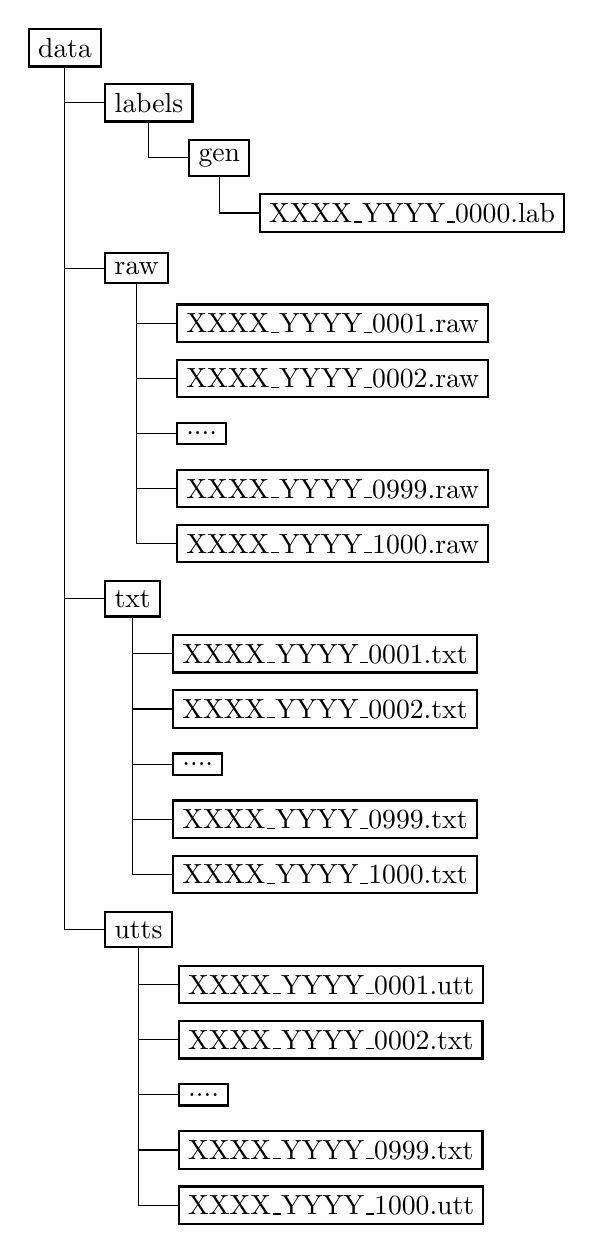
\begin{tikzpicture}[grow via three points={one child at (0.5,-0.7) and two children at (0.5,-0.7) and (0.5,-1.4)},	edge from parent path={(\tikzparentnode.south) |- (\tikzchildnode.west)}]
	\node {data}
	child { node {labels}
		child { node {gen}
			child { node {XXXX\_YYYY\_0000.lab}}
		}
	}
	child [missing] {}
	child [missing] {}
	child { node {raw}
		child { node {XXXX\_YYYY\_0001.raw}}
		child { node {XXXX\_YYYY\_0002.raw}}
		child { node {....}}
		child { node {XXXX\_YYYY\_0999.raw}}
		child { node {XXXX\_YYYY\_1000.raw}}
	}
	child [missing] {}
	child [missing] {}
	child [missing] {}
	child [missing] {}
	child [missing] {}
	child { node {txt}
		child { node {XXXX\_YYYY\_0001.txt}}
		child { node {XXXX\_YYYY\_0002.txt}}
		child { node {....}}
		child { node {XXXX\_YYYY\_0999.txt}}
		child { node {XXXX\_YYYY\_1000.txt}}
	}
	child [missing] {}
	child [missing] {}
	child [missing] {}
	child [missing] {}
	child [missing] {}
	child { node {utts}
		child { node {XXXX\_YYYY\_0001.utt}}
		child { node {XXXX\_YYYY\_0002.txt}}
		child { node {....}}
		child { node {XXXX\_YYYY\_0999.txt}}
		child { node {XXXX\_YYYY\_1000.utt}}
	};
	\end{tikzpicture}
	
	\newpage
	Untuk mempermudah, berikut dijelaskan contoh:
	
	\begin{enumerate}
		\item Hanya ada satu data set, semisal:
		
		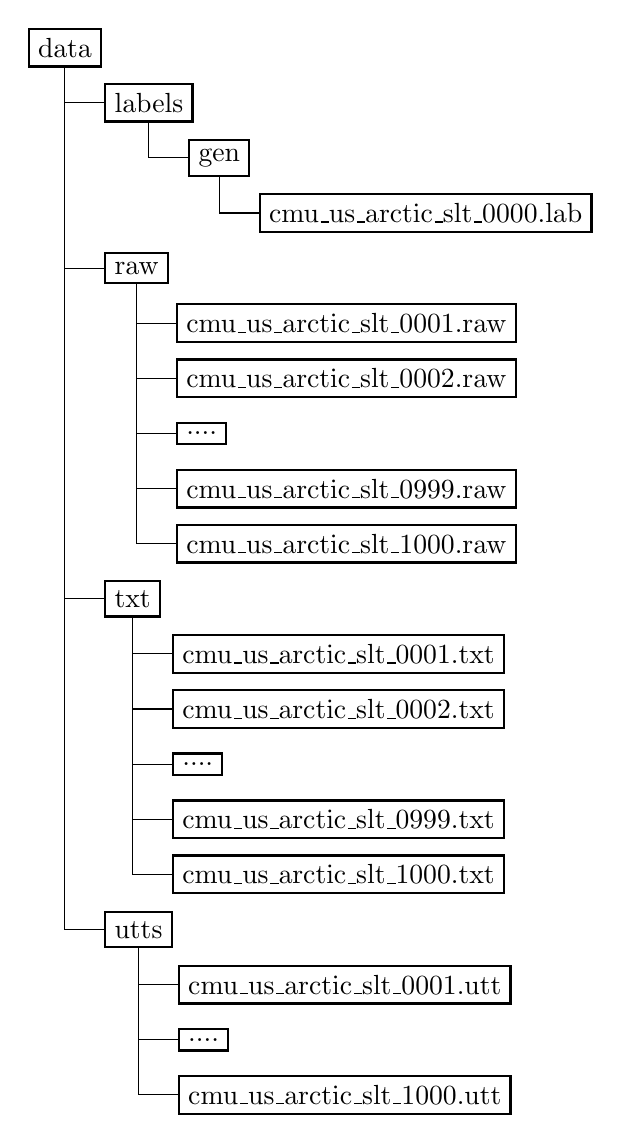
\begin{tikzpicture}[grow via three points={one child at (0.5,-0.7) and two children at (0.5,-0.7) and (0.5,-1.4)},	edge from parent path={(\tikzparentnode.south) |- (\tikzchildnode.west)}]
		\node {data}
		child { node {labels}
			child { node {gen}
				child { node {cmu\_us\_arctic\_slt\_0000.lab}}
			}
		}
		child [missing] {}
		child [missing] {}
		child { node {raw}
			child { node {cmu\_us\_arctic\_slt\_0001.raw}}
			child { node {cmu\_us\_arctic\_slt\_0002.raw}}
			child { node {....}}
			child { node {cmu\_us\_arctic\_slt\_0999.raw}}
			child { node {cmu\_us\_arctic\_slt\_1000.raw}}
		}
		child [missing] {}
		child [missing] {}
		child [missing] {}
		child [missing] {}
		child [missing] {}
		child { node {txt}
			child { node {cmu\_us\_arctic\_slt\_0001.txt}}
			child { node {cmu\_us\_arctic\_slt\_0002.txt}}
			child { node {....}}
			child { node {cmu\_us\_arctic\_slt\_0999.txt}}
			child { node {cmu\_us\_arctic\_slt\_1000.txt}}
		}
		child [missing] {}
		child [missing] {}
		child [missing] {}
		child [missing] {}
		child [missing] {}
		child { node {utts}
			child { node {cmu\_us\_arctic\_slt\_0001.utt}}
			child { node {....}}
			child { node {cmu\_us\_arctic\_slt\_1000.utt}}
		};
		\end{tikzpicture}
		
		Maka perintah konfigurasi dengan menentukan DATASET dan SPEAKER nya:
		
		\begin{minted}[frame=lines,framesep=2mm,fontsize=\footnotesize,bgcolor=LightGray]{bash}
chmod a+x configure
./configure \
--with-fest-search-path=$TOOLS_DIR/festival/examples \
--with-sptk-search-path=$TOOLS_DIR/bin \
--with-hts-search-path=$TOOLS_DIR/bin \
--with-hts-engine-search-path=$TOOLS_DIR/bin \
DATASET=cmu_us_arctic SPEAKER=slt
		\end{minted}
		
		\newpage
		\item Dua atau lebih dataset, semisal:
		
		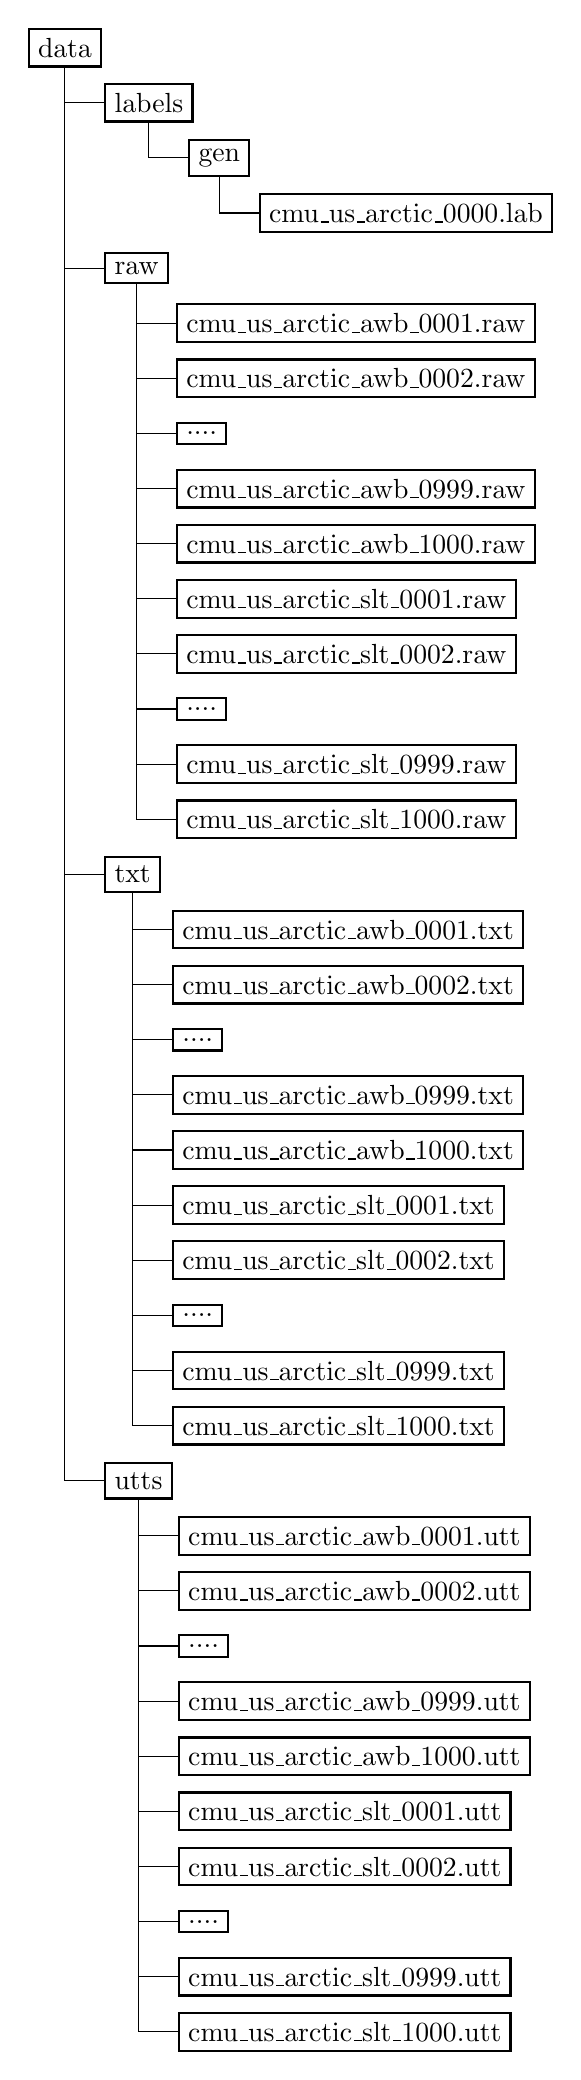
\begin{tikzpicture}[grow via three points={one child at (0.5,-0.7) and two children at (0.5,-0.7) and (0.5,-1.4)},	edge from parent path={(\tikzparentnode.south) |- (\tikzchildnode.west)}]
		\node {data}
		child { node {labels}
			child { node {gen}
				child { node {cmu\_us\_arctic\_0000.lab}}
			}
		}
		child [missing] {}
		child [missing] {}
		child { node {raw}
			child { node {cmu\_us\_arctic\_awb\_0001.raw}}
			child { node {cmu\_us\_arctic\_awb\_0002.raw}}
			child { node {....}}
			child { node {cmu\_us\_arctic\_awb\_0999.raw}}
			child { node {cmu\_us\_arctic\_awb\_1000.raw}}
			child { node {cmu\_us\_arctic\_slt\_0001.raw}}
			child { node {cmu\_us\_arctic\_slt\_0002.raw}}
			child { node {....}}
			child { node {cmu\_us\_arctic\_slt\_0999.raw}}
			child { node {cmu\_us\_arctic\_slt\_1000.raw}}
		}
		child [missing] {}
		child [missing] {}
		child [missing] {}
		child [missing] {}
		child [missing] {}
		child [missing] {}
		child [missing] {}
		child [missing] {}
		child [missing] {}
		child [missing] {}
		child { node {txt}
			child { node {cmu\_us\_arctic\_awb\_0001.txt}}
			child { node {cmu\_us\_arctic\_awb\_0002.txt}}
			child { node {....}}
			child { node {cmu\_us\_arctic\_awb\_0999.txt}}
			child { node {cmu\_us\_arctic\_awb\_1000.txt}}
			child { node {cmu\_us\_arctic\_slt\_0001.txt}}
			child { node {cmu\_us\_arctic\_slt\_0002.txt}}
			child { node {....}}
			child { node {cmu\_us\_arctic\_slt\_0999.txt}}
			child { node {cmu\_us\_arctic\_slt\_1000.txt}}
		}
		child [missing] {}
		child [missing] {}
		child [missing] {}
		child [missing] {}
		child [missing] {}
		child [missing] {}
		child [missing] {}
		child [missing] {}
		child [missing] {}
		child [missing] {}
		child { node {utts}
			child { node {cmu\_us\_arctic\_awb\_0001.utt}}
			child { node {cmu\_us\_arctic\_awb\_0002.utt}}
			child { node {....}}
			child { node {cmu\_us\_arctic\_awb\_0999.utt}}
			child { node {cmu\_us\_arctic\_awb\_1000.utt}}
			child { node {cmu\_us\_arctic\_slt\_0001.utt}}
			child { node {cmu\_us\_arctic\_slt\_0002.utt}}
			child { node {....}}
			child { node {cmu\_us\_arctic\_slt\_0999.utt}}
			child { node {cmu\_us\_arctic\_slt\_1000.utt}}
		};
		\end{tikzpicture}
		
		Maka wajib ditentukan salah satu data mana yang digunakan agar tidak rancu.
		
		Semisal apakah akan menggunakan pembicara AWB:
		
		\begin{minted}[frame=lines,framesep=2mm,fontsize=\footnotesize,bgcolor=LightGray]{bash}
chmod a+x configure
./configure \
--with-fest-search-path=$TOOLS_DIR/festival/examples \
--with-sptk-search-path=$TOOLS_DIR/bin \
--with-hts-search-path=$TOOLS_DIR/bin \
--with-hts-engine-search-path=$TOOLS_DIR/bin \
DATASET=cmu_us_arctic SPEAKER=awb
		\end{minted}

		Atau pembicara SLT (harus salah satu):
		\begin{minted}[frame=lines,framesep=2mm,fontsize=\footnotesize,bgcolor=LightGray]{bash}
chmod a+x configure
./configure \
--with-fest-search-path=$TOOLS_DIR/festival/examples \
--with-sptk-search-path=$TOOLS_DIR/bin \
--with-hts-search-path=$TOOLS_DIR/bin \
--with-hts-engine-search-path=$TOOLS_DIR/bin \
DATASET=cmu_us_arctic SPEAKER=slt
		\end{minted}
		
	\end{enumerate}
	
	\newpage
	\subsection{Tools EnVars}
	
	Pengulangan untuk mempermudah mengingat set EnVars ini akan sering dipanggil.
	
	\begin{minted}[frame=lines,framesep=2mm,fontsize=\footnotesize,bgcolor=LightGray]{bash}
export TOOLS_DIR=~/.hts_sptk

export PATH=$TOOLS_DIR/bin:$PATH
export PATH=$TOOLS_DIR/festival/bin:$PATH
export PATH=$TOOLS_DIR/speech_tools/bin:$PATH

export FESTVOXDIR=$TOOLS_DIR/festvox
export FESTDIR=$TOOLS_DIR/festival
export ESTDIR=$TOOLS_DIR/speech_tools

export PATH=$FESTDIR/examples:$PATH
	\end{minted}
	
	\subsection{Unduh Github}
	
	Untuk memperoleh file atau folder dari Github memiliki beberapa cara,
	namun disini hanya dijelaskan 2 saja, 
	yaitu dengan cloning dan download blob.
	
	Sebagai contoh, disini akan digunakan contoh repository:\\
	\url{https://github.com/mekatronik-achmadi/hts_grapheme}
	
	\subsubsection{Cloning Git}
	
	Dengan menggunakan metode cloning, dapat didownload seluruh struktur file/folder suatu repository.
	Selain file/folder, akan didapatkan juga log/commit repository tersebut. 
	Agar dapat melakukan cloning, diperlukan program \textbf{Git}.
	Untuk instal Git di Ubuntu (dibutuhkan internet dan hak akses root/sudo):
	\begin{minted}[frame=lines,framesep=2mm,fontsize=\footnotesize,bgcolor=LightGray]{bash}
sudo apt-get install git
	\end{minted}
	
	dan untuk Arch-Linux (dibutuhkan internet dan hak akses root/sudo):
	\begin{minted}[frame=lines,framesep=2mm,fontsize=\footnotesize,bgcolor=LightGray]{bash}
sudo pacman -S git
	\end{minted}
	
	Langkah cloning:
	\begin{enumerate}
		\item Buka jendela terminal/shell baru.
		
		\item Semisal alamat URL repository adalah:\\
		\url{https://github.com/mekatronik-achmadi/hts_grapheme} \\
		Maka perintah cloning:
		\begin{minted}[frame=lines,framesep=2mm,fontsize=\footnotesize,bgcolor=LightGray]{bash}
git clone https://github.com/mekatronik-achmadi/hts_grapheme
		\end{minted}
		
		\item Tunggu proses.
		
		\item Repository telah ter-cloning di folder \textbf{hts\_grapheme/}.
		\begin{minted}[frame=lines,framesep=2mm,fontsize=\footnotesize,bgcolor=LightGray]{bash}
tree hts_grapheme/
		\end{minted}
		
	\end{enumerate}
	
	\newpage
	\subsubsection{Download Blob}
	
	Dengan menggunakan metode ini, dapat didownload spesifik file/folder,
	tanpa harus mendownload seluruh repository.
	Yang dibutuhkan hanyalah alamat URL file/folder yang ada di server Github.
	
	Sebagai contoh disini, akan di download folder \textbf{utt2lab} beserta seluruh isinya.
	Alamat di server github adalah:\\
	\url{https://github.com/mekatronik-achmadi/hts_grapheme/tree/master/scripts/utt2lab}
	
	Berikut langkahnya:
	\begin{enumerate}
		\item Buka situs DownGit.
		Salah satunya yang dibangun oleh user minhaskamal.\\
		\url{https://minhaskamal.github.io/DownGit/}
		
		\begin{figure}[!ht]
			\centering
			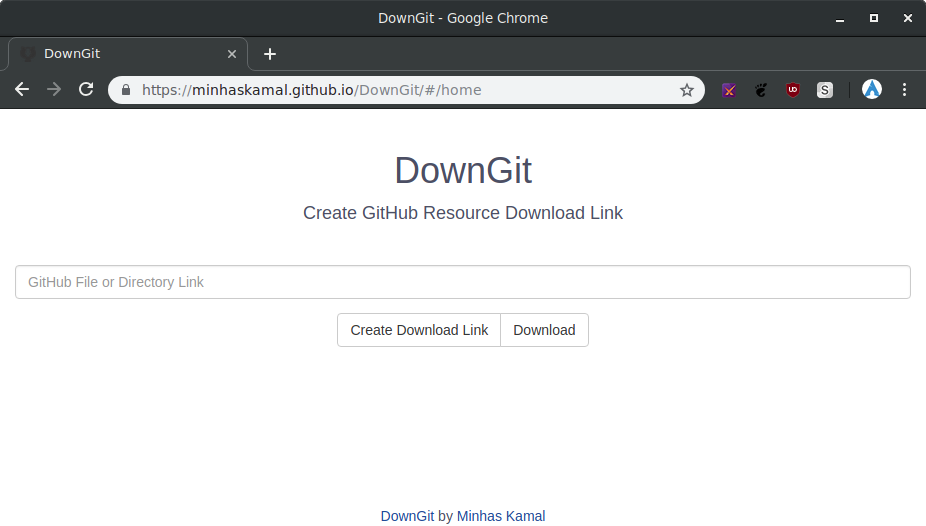
\includegraphics[width=450pt]{downgit.png}
		\end{figure}
		
		\item Salin alamat URL folder \textbf{utt2lab} ke kolom panjang kosong di situs DownGit.
		
		\item Tekan Enter.
		
		\item File/folder akan terdownload dalam arsip Zip.
	\end{enumerate}

	\subsection{Script Tambahan}
	
	Tesedia di repository beberapa skrip Bash tambahan untuk mempermudah salin atau hapus file.
	Skrip tersedia di alamat:\\
	\url{https://github.com/mekatronik-achmadi/hts_grapheme/tree/master/scripts}
	
	Skrip tambahan yang tersedia antara lain:
	\begin{itemize}
		\item \textbf{copy\_loop.sh}.\\
		Dapat digunakan untuk membantu salin file berdasarkan nama dan rentang angka spesifik.
		
		\item \textbf{remove\_unused.sh}.\\
		Dapat digunakan untuk membantu menghapus file berdasarkan angka spesifik.
		
		\item \textbf{run\_synthesis.sh}.\\
		Dapat digunakan untuk menjalankan proses synthesis tanpa memasukkan perintah satu per satu.
		
		\item \textbf{install\_ubuntu.sh} dan \textbf{install\_archlinux.sh}.\\
		Dapat digunakan untuk membantu instalasi paket tools di distro Ubuntu dan Arch-Linux.
	\end{itemize}
	
	\newpage
	\section{Troubleshoot}
	Berikut beberapa trouble yang telah dipahami:
	
	\begin{itemize}
		\item Segmen Label phonem yang kurang dari 3 di txt/raw/utts.
		Contoh:
		\begin{minted}[frame=lines,framesep=2mm,fontsize=\footnotesize,bgcolor=LightGray]{text}
 Number of owners = 1
SegLab   :  sy
maxIter  :  20
epsilon  :  0.000100
minSeg   :  1
Updating :  Means Variances MixWeights/DProbs TransProbs

- system is PLAIN
ERROR [+2121]  HInit: Too Few Observation Sequences [0]
		\end{minted}
		
		Dari contoh terlihat bahwa phonem \textbf{sy} pada data raw/txt/utts untuk training model kurang dari 3.
		Phonem yang kurang terlihat pada nilai \textbf{SegLab}.
		
		Solusi: Tambah data training (raw/txt/utts) yang memuat phone tersebut.
		
		\item File full-context label yang akan disynthesis tidak tersedia.
		Contoh:
		\begin{minted}[frame=lines,framesep=2mm,fontsize=\footnotesize,bgcolor=LightGray]{text}
sed: can't read labels/gen/*.lab: No such file or directory
Makefile:311: recipe for target 'list' failed
make[1]: *** [list] Error 2
		\end{minted}
		
		Solusi: cek folder \textbf{data/labels/gen/} apakah telah terisi full-context label.
		
		\item Ukuran data synthesis terlalu besar.
		Contoh:
		\begin{minted}[frame=lines,framesep=2mm,fontsize=\footnotesize,bgcolor=LightGray]{text}
x2x : warning: input data is over the range of type 'short'!
		\end{minted}
		
		Solusi: Cek konten label untuk synthesis dan berdoa.
		
		\item Alignment yang tidak pas.
		Contoh:
		\begin{minted}[frame=lines,framesep=2mm,fontsize=\footnotesize,bgcolor=LightGray]{text}
Unable to traverse 175 states in 77 frames
WARNING [-7324]  StepBack: Bad data or over pruning
in /home/elokhts/.hts_sptk/bin/HERest
		\end{minted}
		
		Atau:
		\begin{minted}[frame=lines,framesep=2mm,fontsize=\footnotesize,bgcolor=LightGray]{text}
WARNING [-9999]  HSMMAlign: No tokens survived to final node of network at beam 2000
		\end{minted}
		
		Atau:
		\begin{minted}[frame=lines,framesep=2mm,fontsize=\footnotesize,bgcolor=LightGray]{text}
Making data, labels, and scp from vibid_fena_0465.lab for GV...
Cannot open No such file or directory at scripts/Training.pl line 1192, <SCP> line 365.
		\end{minted}

		Solusi: Cek konten utterance untuk training dan berdoa.
		
	\end{itemize}
	
	Jika ditemukan masalah lain, solusinya berdoalah semoga masalah tersebut selesai dengan sendirinya.
	
	\newpage
	\mbox{}
	
	\newpage
	\section{Website}
	
	Berikut URL Website yang bermanfaat:
	\begin{itemize}
		\item Repository Github untuk panduan ini:\\
		\url{https://github.com/mekatronik-achmadi/hts_grapheme}
		
		\item Sumber informasi utama:\\
		\url{https://google.com}
		
	\end{itemize}

	\newpage
	\mbox{}
	
	\newpage
	\section{Referensi}
	
	\url{https://google.com}
	
	\newpage
	\mbox{}
	
\end{document}
